\subsection{Business Continuity Process}

Un piano per la continuazione del business si suddivide nei seguenti passi:
\begin{enumerate}
  \item Attuazione dell'\textit{Business Impact Analysis}
  \item Privatizzazione dei servizi di supporto critici per i servizi di 
  business
  \item Determinazione del processo della modalità alternativa per i servizi 
  critici e vitali
  \item Sviluppare il piano di \textit{Disaster Recovery} per i servizi di 
  recupero IS
  \item Sviluppo di tipo BCP per le operazioni di recupero e continuazione del 
  business
  \item Test dei piani
  \item Mantenimento dei piani
\end{enumerate}

\subsection{Esercizi}

Gli esercizi si trovano nella sezione \ref{EsBCDR1}.

\section{Disaster recovery testing}

Un incidente non viene dichiarato immediatamente, ma c'è una procedura da 
rispettare. Quando una situazione di incidente è dichiarata l'incolumità fisica 
è la prima a essere presa in considerazione. Gli \textit{Stackeholders} sono 
subito contattati, mentre l'ufficio stampa si occupa di dichiarare l'incidente. 
Questa parte è molto delicata, e il danno dev'essere spiegato in maniera da non 
costituire una brutta pubblicità per l'azienda.

L'ufficio IT entra in azione dopo tutte queste procedure preliminari sono 
annunciate, e comincia ad agire per risolvere il problema.

\subsection{Preparazione di un piano di recupero}

La vita delle persone viene messa sempre in primo piano. Viene poi definito chi 
deve fare cosa. Le copie del piano di recupero devono essere distribuite in 
diverse locazioni per evitare che possano essere distrutte.

\subsubsection{Responsabilità in un piano di recupero}

All'interno dell'azienda parte del personale ricopre dei ruoli dal punto di 
vista della sicurezza delle persone, e sono pronti ad agire in caso una 
situazione di pericolo si manifesti.

Ad esempio, in ogni piano di una struttura (come un ufficio o un edificio 
pubblico) dovrebbe essere presente una persona che si incarichi di controllare 
ogni stanza per verificare l'assenza di persone in difficoltà in caso di una 
evacuazione d'emergenza.

\subsection{Documenti di un piano di recupero}

% TODO: copiare la tabella

% Please add the following required packages to your document preamble:
% \usepackage{graphicx}
\begin{table}[H]
\centering
\label{my-label}
\resizebox{\textwidth}{!}{%
\begin{tabular}{|l|p{5cm}|p{5cm}|}
\hline
\textbf{Focus}                   & \textbf{IT}                                   
                                              & \textbf{Business}                
                                                                    \\ \hline
Evento di recupero      & Piano di recupero del disastro. Procedure per 
recuperare in modalità alternativa   & Piano di recupero del Business. Recupero 
del business dopo un disastro                      \\ \hline
                        & Piano di contingenza IT: recupero della maggior parte 
delle applicazioni o sistemi & Piano di emergenza per gli occupanti: proteggere 
la vita e le risorse sotto pericolo fisico \\ \hline
                        & Piano di risposta per un incidente cibernetico 
malizioso                           & Piano di comunicazione di crisi: da un 
report della situazione al pubblico e al personale   \\ \hline
Continuità del business &                                                        
                            & Piano di continuità del business                   
                                         \\ \hline
                        &                                                        
                            & Piano di continuità delle operazioni in caso di 
interruzioni prolungate                     \\ \hline
\end{tabular}%
}
\caption{Lista dei vari documenti di un piano di recupero}
\end{table}

\subsection{\textit{Mean Time Between Failure}}

Detto anche MTBF è la somma del \textit{Mean Time to Repair} (MTTR) più il 
\textit{Mean Time To Fail} (MTTF).

\begin{figure}[H]
 \centering
 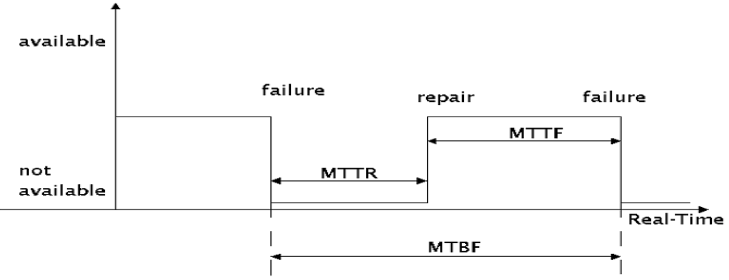
\includegraphics[scale=0.5]{mtbf}
 \caption{Grafico rappresentate i vari valori di un MTBF, MTTR e MTTF}
\end{figure}


L'affidabilità può essere misurata. Un tipica misura è quella detta del 
\textit{5 9s}, ovvero del $99.999\%$ di \textit{uptime}, ovvero 5 minuti e 
mezzo di fallimento all'anno del servizio.

\subsection{Esecuzione del test}

È l'esecuzione del piano per verificarne il suo funzionamento.
Il test viene effettuato in questo ordine:
\begin{enumerate}
  \item \textbf{Desk-Based Evaluation/Paper test} \\
  Un gruppo comincia a seguire i passi della procedura e li esegue a mano
  \item \textbf{Preparedness Test} \\
  Una o più parti dell'intero test vengono eseguite.
  \item \textbf{Full Operational Test} \\
  Simulazione di un disastro completo
\end{enumerate}

\subsubsection{Tipologie di test per il Business Continuity}

Esistono diverse tipologie di test per il \textit{Business Continuity}:
\begin{itemize}
  \item Checklist Review \\
  Rivisitazione per piano di copertura. Tutti i piani importanti sono coperti?
  \item Structured Walkthrough \\
  Rivisitazione di tutti gli aspetti del piano, spesso guardando tutti gli 
  scenari
  \item Simulation Test \\
  Esecuzione del piano basato specificamente per uno scenario, senza un sito 
  alternativo
  \item Parallel Test \\
  Viene azionato la struttura alternativa fuori dal sito, senza 
  interrompere il funzionamento del sito regolare
  \item Full-Interruption \\
  Si passa alla modalità alternativa da quella regolare, per verificare che 
  tutto sia funzionante.
\end{itemize}

\subsubsection{Obiettivi del testing}

Il testing del piano deve risultare in un recupero con successo delle 
infrastrutture e dei processi di \textit{business}

\paragraph*{Vantaggi} Ci sono i seguenti vantaggi nell'eseguire il testing:
\begin{itemize}
  \item Identificazione di probabili errori
  \item Verifica delle assunzioni fatte
  \item Verifica dei tempi
  \item Allenamento e coordinamento dello staff
\end{itemize}

\subsubsection{Procedure del testing}

I test sono inizialmente semplici e poi diventano man mano sempre più complessi 
con il tempo.


\begin{figure}[H]
 \centering
 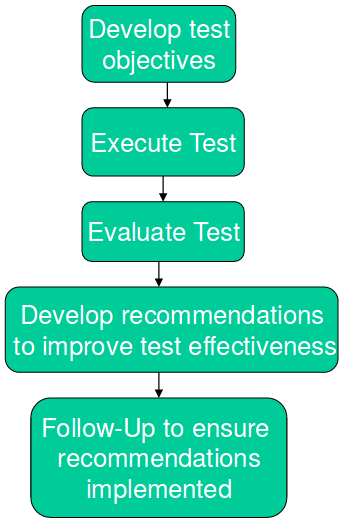
\includegraphics[scale=0.5]{tp}
 \caption{Varie procedure del testing}
\end{figure}

Includono di solito una terza parte indipendente, per poter permetterne una 
migliore osservazione.

Dalla valutazione del test si ottengono quelli che sono i \textbf{punti di 
miglioramento}, che devono essere effettivamente messi in pratica.

\paragraph*{Passi del test} Esistono diversi passi del test. C'è la sua 
preparazione, l'esecuzione del test e la pulizia dopo-test. Importante è 
ricordarsi di eseguire una pulizia dei dati dopo l'esecuzione del test, ma di 
quelli che non sono importanti per la sua valutazione (altrimenti il test 
sarebbe inutile).

\subsubsection{\textit{Gap Analysis}}

Una \textit{gap analysis} è relativa a un obiettivo che un'azienda si pone 
rispetto al punto in cui è, ed è necessaria affinché una azienda possa 
migliorare se stessa. Quelli che sono più controllati sono i 
processi\footnote{Importante è il PDCA (miglioramento continuo della qualità 
dei processi).}, perché le persone sono quelle che sono più difficili da 
``modificare'' ed essere migliorate.

\subsection{Auditing di un BCP}

Sono presenti diversi step da controllare, che possono essere:
\begin{itemize}
  \item Include la BIA?
  \item È il BCP in linea con i goals del business, sono effettivi o moderni?
  \item È chiaro chi dovrà svolgere cosa?
  \item Sono tutti competenti? Accettano volentieri questo ruolo?
  \item DRP è mantenuto e dettagliato?
  \item Le procedure di backup e di recupero sono seguite?
\end{itemize}

% Manca parte sull'assicurazione

\section{Riassunto dei controlli principali per i controlli di sicurezza BC}

\begin{itemize}
  \item RAID
  \item Diversi tipi di backup
  \item Diversi tipi di protezione sulla rete
  \item Siti alternativi in caso di problemi
  \item Applicazione di test
  \item Assicurazione
\end{itemize}

\section{Esercizi}

The FIRST thing that should be done when you discover an intruder has hacked 
into your computer system is to:
\begin{itemize}
  \item Disconnect the computer facilities from the computer network to 
  hopefully disconnect the attacker
  \item Power down the server to prevent turther loss of confidentiality and 
  data itegrity
  \item Call the manager
  \item Follow the directions of the Incident Response Plan (risposta esatta)
\end{itemize}

% Altro esercizio

During an audia of the business continuity plan, the finding of MOST convern is:
\begin{itemize}
  \item The phone tree has not been double-checked in 6 months
  \item The business impact analysis has not been updated this year
  \item A test of the  backup-recovery system is not performed regularly 
  (risposta esatta)
  \item The backup library site lacks a UPS
\end{itemize}